%%%%%%%%%%%%%%%%%%%%%%%%%%%%%%%%%%%%%%%%%
% Beamer Presentation
% LaTeX Template
% Version 1.0 (10/11/12)
%
% This template has been downloaded from:
% http://www.LaTeXTemplates.com
%
% License:
% CC BY-NC-SA 3.0 (http://creativecommons.org/licenses/by-nc-sa/3.0/)
%
%%%%%%%%%%%%%%%%%%%%%%%%%%%%%%%%%%%%%%%%%

%----------------------------------------------------------------------------------------
%	PACKAGES AND THEMES
%----------------------------------------------------------------------------------------

\documentclass[aspectratio=149]{beamer}
\usefonttheme[onlymath]{serif}


\mode<presentation> {

% The Beamer class comes with a number of default slide themes
% which change the colors and layouts of slides. Below this is a list
% of all the themes, uncomment each in turn to see what they look like.

\usetheme{default}
%\usetheme{AnnArbor}
%\usetheme{Antibes}
%\usetheme{Bergen}
%\usetheme{Berkeley}
%\usetheme{Berlin}
%\usetheme{Boadilla}
%\usetheme{CambridgeUS}
%\usetheme{Copenhagen}
%\usetheme{Darmstadt}
%\usetheme{Dresden}
%\usetheme{Frankfurt}
%\usetheme{Goettingen}
%\usetheme{Hannover}
%\usetheme{Ilmenau}
%\usetheme{JuanLesPins}
%\usetheme{Luebeck}
%\usetheme{Malmoe}
%\usetheme{Marburg}
%\usetheme{Montpellier}
%\usetheme{PaloAlto}
%\usetheme{Pittsburgh}
%\usetheme{Rochester}
%\usetheme{Singapore}
%\usetheme{Szeged}
%\usetheme{Warsaw}

% As well as themes, the Beamer class has a number of color themes
% for any slide theme. Uncomment each of these in turn to see how it
% changes the colors of your current slide theme.

%\usecolortheme{albatross}
%\usecolortheme{beaver}
\usecolortheme{spruce}
%\usecolortheme{beetle}
%\usecolortheme{crane}
%\usecolortheme{dolphin}
%\usecolortheme{dove}
%\usecolortheme{fly}
%\usecolortheme{lily}
%\usecolortheme{orchid}
%\usecolortheme{rose}
%\usecolortheme{seagull}
%\usecolortheme{seahorse}
%\usecolortheme{whale}
%\usecolortheme{wolverine}

%\setbeamertemplate{footline} % To remove the footer line in all slides uncomment this line
%\setbeamertemplate{footline}[page number] % To replace the footer line in all slides with a simple slide count uncomment this line

%\setbeamertemplate{navigation symbols}{} % To remove the navigation symbols from the bottom of all slides uncomment this line
}

\usepackage{graphicx} % Allows including images
\usepackage{booktabs} % Allows the use of \toprule, \midrule and \bottomrule in tables
\usepackage{verbatim}

\usepackage{mathtools} 
\usepackage{amssymb}
\usepackage{mathrsfs}
\usepackage{amsmath}
\usepackage{bm}

\usepackage{ragged2e}
\usepackage{etoolbox}
\usepackage{lipsum}

\usepackage{siunitx,booktabs}
\usepackage{pifont}
\usepackage{array}
\usepackage{tabu,booktabs}
\usepackage{tikz}
\usetikzlibrary{arrows,shapes}

\setbeamertemplate{enumerate items}[circle]
\usepackage{tikz}

\newcommand\mynum[1]{
  \usebeamercolor{enumerate item}
  \tikzset{beameritem/.style={circle,inner sep=0,minimum size=2ex,text=enumerate item.bg,fill=enumerate item.fg,font=\footnotesize}}%
  \tikz[baseline=(n.base)]\node(n)[beameritem]{#1};
}

\newcommand\mynumm[1]{
  \usebeamercolor{enumerate item}
  \tikzset{beameritem/.style={rectangle,inner sep=0,minimum size=2ex,text=enumerate item.bg,fill=enumerate item.fg,font=\footnotesize}}%
  \tikz[baseline=(n.base)]\node(n)[beameritem]{#1};
}

\def\Put(#1,#2)#3{\leavevmode\makebox(0,0){\put(#1,#2){#3}}}

\setbeamertemplate{footline}[frame number]

%----------------------------------------------------------------------------------------
%	TITLE PAGE
%----------------------------------------------------------------------------------------

\title{ Subsidized Housing as a Place-Based Policy: \\ Evidence from South Africa } % The short title appears at the bottom of every slide, the full title is only on the title page

\author{Ben Bradlow, Stefano Polloni, Will Violette} 

 % Your institution as it will appear on the bottom of every slide, may be shorthand to save space

\date{May 2018} %\today} % Date, can be changed to a custom date

\begin{document}

\beamertemplatenavigationsymbolsempty

\begin{frame}
\titlepage % Print the title page as the first slide
\end{frame}

%\begin{frame}
%\frametitle{Overview} % Table of contents slide, comment this block out to remove it
%\tableofcontents % Throughout your presentation, if you choose to use \section{} and \subsection{} commands, these will automatically be printed on this slide as an overview of your presentation
%\end{frame}

%----------------------------------------------------------------------------------------
%	PRESENTATION SLIDES
%----------------------------------------------------------------------------------------
\section{Introduction}
%------------------------------------------------

\begin{frame}
\frametitle{Slums and Development}

% In developing countries, 30\% of urban pop live in slums (UN, 2015)

\begin{itemize}
  \item Slum externalities $\rightarrow$ lasting poverty traps (Marx, 2013) 
    \begin{itemize}
      \item Poor infrastructure, high crime, health externalities
      \item Weak incentives to invest in housing/public goods
    \end{itemize}  
\vspace{.2cm}
%\pause
  \item \textbf{Public Housing} $\rightarrow$ primary government response
\end{itemize}
%    \pause
\begin{enumerate}
  \item Direct Recipient Impacts
    \begin{itemize}
      \item Health, Wellbeing, Employment, Redistribution \\ \footnotesize{(Cateneo et al. [2009], Franklin et al. [2016], Galiani et al. [2017])}
    \end{itemize}
% ``key strategy for poverty alleviation'' {\footnotesize{South Africa}}
%    \pause
    \vspace{.1cm}
\item Neighborhood Development
  \begin{itemize}
    \item ``combating crime, promoting social cohesion... spatial restructuring'' South Africa Dept. of Human Settlements
%    \pause
    \item Little research on spillovers \footnotesize{(Diamond and McQuade (2016))}
  \end{itemize}
\end{enumerate}

\begin{itemize}
  \item \textbf{Question} \\ 
  \vspace{.1cm}
  What are the spillovers from public housing in developing contexts?
\end{itemize}
% ``combating crime, promoting social cohesion... spatial restructuring,'' {\footnotesize{South Africa}}
\end{frame}

%------------------------------------------------

\begin{frame}
\frametitle{This Paper}

\begin{itemize}
  \item \textbf{Question} \\ 
  \vspace{.1cm}
  What are the spillovers from public housing in developing contexts?
  \vspace{.1cm}
    \begin{itemize}
      \item \textbf{Positive:} Incentivize investments in housing/public goods
      \item \textbf{Negative:} Crowd in slum growth
    \end{itemize}

%\pause
\vspace{1mm}
\item \textbf{Approach} \\ Leverage precise timing/geography of large housing projects
\vspace{1mm}
\item \textbf{New Data and Setting} \\ 172 projects in South Africa combined with GPS property transactions and slum growth data
\vspace{1mm}
\item \textbf{Initial Findings} \\ Housing projects depress home prices by 5\% within 300 meters
\begin{itemize}
  \item heterogeneity
  \item ballpark estimates
\end{itemize}
\end{itemize}

\end{frame}


%------------------------------------------------

\begin{frame}
\frametitle{Public Housing in South Africa}
  \begin{itemize}
      \item Over 4.3 million houses since 1994 (13\% of pop.)
%      \item Houses 13\% of the population
%      \item Single-story, two-room (30-40$\text{m}^2$) dwellings
      \begin{itemize}
        \item 50 to 500 houses per project
      \end{itemize}
  \end{itemize}
    %%% insert picture


\begin{itemize}
        \item Who gets a house?
      \begin{itemize}
        \item Official Policy: 
          \begin{itemize}
            \item National/provincial waiting lists
            \item No resale within 7 years
            \item Citizens, new homeowners, married or dependents, inc/month $<$R3,500
          \end{itemize}
        \item In Practice:
          \begin{itemize}
            \item Waiting lists/eligibility weakly enforced
            \item Only 82\% of houses occupied by initial owners within 5 yrs
          \end{itemize}
      \end{itemize}
\end{itemize}
\end{frame}

%------------------------------------------------

\begin{frame}
\frametitle{Where are these houses built?}

\begin{enumerate}
  \item \textbf{Greenfield projects} on undeveloped land near slums
  \item \textbf{In-Situ upgrading} replacing existing slums
\end{enumerate}

\begin{itemize}
  \item insert picture here
\end{itemize}

\begin{itemize}
  \item Projects are fully serviced (roads, water, sanitation, electricity)
\end{itemize}
    %%% insert small maps of pre-post periods (with cherry picked examples) (with google maps? or bblu?) or find good sattelite from an evaluation?

\end{frame}

%------------------------------------------------



\begin{frame}
\frametitle{Conceptual Framework: Public Housing Impacts}

\begin{enumerate}
  \item \textbf{Amenity Effect:} Upgrading housing stock/services
    \begin{itemize}
        \item Increase value of neighboring homes (Rossi-Hansberg [2010])
    \end{itemize}
\vspace{.2cm} 

  \item \textbf{Crowd-In Slums:} Reduce costs of informal housing
    \begin{itemize}
        \item Overburden services, health/crime externalities
        \item Reduce value of nearby houses
    \end{itemize}
\vspace{.2cm}

  \item \textbf{Demographic Effect:} New people in the neighborhood
    \begin{itemize}
        \item Taste-based discrimination (Diamond and McQuade [2016])
    \end{itemize}
\end{enumerate}

%\begin{enumerate}
%  \item Housing externalities  {\small (Rossi-Hansberg [2010]) }
%    \begin{itemize}
%      \item Home value depends on the quality of neighboring homes
%      \item ie. informal dwellings have poor sanitation
%    \end{itemize}
%\vspace{.1cm}
%  \item Demographic externalities
%    \begin{itemize}
%      \item Taste-based discrimination
%      \item Overcrowding $\rightarrow$ crime/health externalities
%    \end{itemize}
%\vspace{.1cm}
%  \item Access to public goods (water, sewer, road infrastructure)
%\end{enumerate}

\end{frame}



%------------------------------------------------



\begin{frame}
\frametitle{Measuring Public Housing and Spillovers}

\begin{itemize}
  \item Focus on Gauteng Province (includes Johannesburg and Pretoria)
\end{itemize}

\begin{enumerate}
\item \textbf{Property Transactions} measure housing projects and price impacts
  \begin{itemize}
    \item 500,000 deeds records (bottom 20\% of formal housing market)
    \item Buyer/seller name, GPS, price, date from 2002-2011
  \end{itemize}
\vspace{.2cm}
\item \textbf{Building Census} identifies slum-growth and in-situ upgrading
  \begin{itemize}
    \item 4 mil. residential buildings (50\% informal) GPS in 2001 and 2011
  \end{itemize}
\vspace{.2cm}
\item \textbf{Population Census} measures demographic and economic impacts
  \begin{itemize}
    \item Full census for 18,000 census blocks in 2001 and 2011
  \end{itemize}
\vspace{.2cm}
\item \textbf{Administrative Data} map projects (construction dates and costs)
  \begin{itemize}
    \item Not comprehensive
    \item Includes planned but unconstructed projects
  \end{itemize}


\end{enumerate}

\end{frame}

%------------------------------------------------

%  
%  
%  \item \textbf{Temporal Clustering:} include cluster with $>$50\% of transactions during modal year


\begin{frame}
\frametitle{Identifying Housing Projects}

\begin{tikzpicture}[overlay]

\onslide<1->\node[overlay,anchor=west,align=left] at (0, 2.5) {    \begin{minipage}{1\textwidth} {\begin{enumerate}
  \item \textbf{Seller Identity:} match government names and housing authorities in seller-names from transactions 
\end{enumerate}}\end{minipage}};

\onslide<2->\node[overlay,anchor=west,align=left] at (0, 1.5) {    \begin{minipage}{1\textwidth} { 
\begin{enumerate}
  \setcounter{enumi}{1}
  \item \textbf{Subsidy Value:} exclude purchase prices R50,000 above subsidy value
\end{enumerate}}\end{minipage}};

\onslide<3->\node[overlay,anchor=west,align=left] at (0, .5) {    \begin{minipage}{1\textwidth} { 
\begin{enumerate}
  \setcounter{enumi}{2}
  \item \textbf{Pre-Existing Formal Dwellings:} exclude land plots with formal structures in 2001 building census
\end{enumerate}}\end{minipage}};

\onslide<4->\node[overlay,anchor=west,align=left] at (0, -.5) {    \begin{minipage}{1\textwidth} { 
\begin{enumerate}
  \setcounter{enumi}{3}
  \item \textbf{Spatial Clustering:} collect nearby houses into projects with density-based clustering algorithm
\end{enumerate}}\end{minipage}};

\onslide<5->\node[overlay,anchor=west,align=left] at (0, -1.5) {    \begin{minipage}{1\textwidth} { 
\begin{enumerate}
  \setcounter{enumi}{4}
  \item \textbf{Temporal Clustering:} include clusters with $>$50\% of transactions during modal year
\end{enumerate}}\end{minipage}};

\onslide<5->\node[overlay,anchor=west,align=left] at (0, -2.6) {    \begin{minipage}{1\textwidth} { 
\begin{itemize}
  \item Overlaps well with completed projects from admin. data
\end{itemize}}\end{minipage}};



\onslide<1>\node[overlay,anchor=west,align=left] at (0, -1) {
\begin{minipage}{1\textwidth} { 
\begin{figure}
\caption{Top 5 Seller Names}
\begin{tabu}{lc}
\toprule
 Seller Name & Observations \\
\midrule
City Of Johannesburg Metropolitan Municipality & 29,087  \\
City Of Johannesburg & 27,672  \\
City Of Tshwane Metropolitan Municipality & 24,780  \\
Ekurhuleni Metropolitan Municipality & 21,758  \\
Gauteng Provincial Housing Advisory Board & 13,058  \\
{\bf Total Observations }& {\bf 549,704}  \\
\bottomrule
\end{tabu}
 
\end{figure}
}\end{minipage}
} ;
% descriptive_statistics.do   program: write_biggest_sellers


\onslide<2>\node[overlay,anchor=west,align=left] at (0, -1.7) { 
\begin{minipage}{1\textwidth} { 
\begin{figure}
\caption{Purchase Price Densities}
 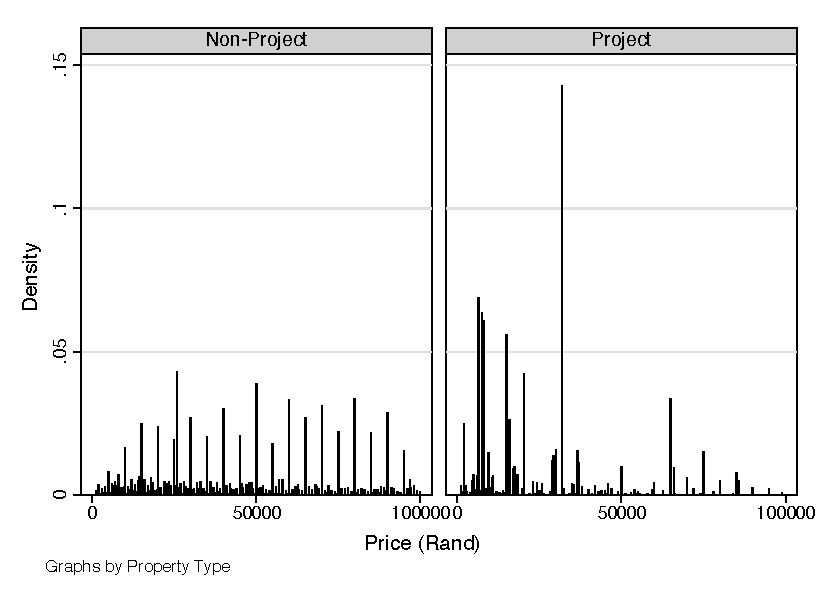
\includegraphics[scale=.53]{price_histogram.pdf} 
\end{figure}
}\end{minipage} 
} ;
% descriptive_statistics.do   program: write_price_histogram


\onslide<4>\node[overlay,anchor=west,align=left] at (2, -2.8) {  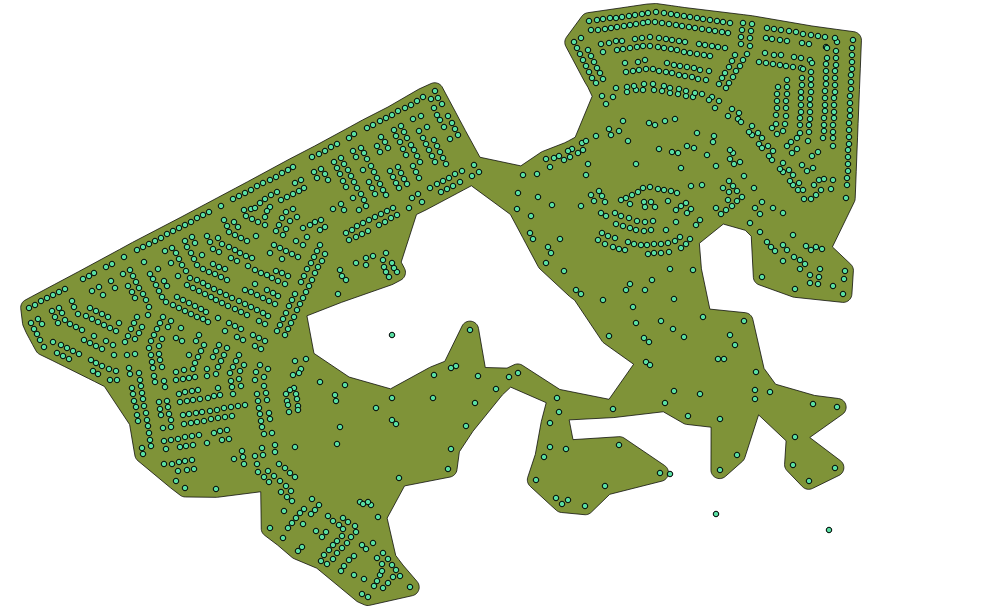
\includegraphics[scale=.16]{rdp_conhull_pic.png}  };
% generated from QGIS


\end{tikzpicture}

\end{frame}





%------------------------------------------------


\begin{frame}
\frametitle{Identifying Planned but Unconstructed Projects}

\begin{enumerate}
  \item Admin. data have ``planned,'' ``proposed,'' ``implementing'' projects
    \begin{itemize}
      \item Exclude projects with identified project transactions
    \end{itemize}

    \vspace{.2cm}

  \item Assign projects an expected completion date
    \begin{itemize}
      \item Fuzzy-string match budget data (with start-dates) on project names
      \item Add avg. diff. between transaction-date and start-date for completed projects
    \end{itemize}
\end{enumerate}

\begin{itemize}
  \item Why are projects canceled/delayed? 
    \begin{itemize}
      \item Legal disputes, service delivery backlogs, funding complications
      \item Delays often exceed 12 years 
    \end{itemize} 
\end{itemize}

\end{frame}


%------------------------------------------------

\begin{frame}
\frametitle{Housing Projects}
\begin{table}
\caption{Housing Projects and Building Growth}
\begin{tabu}{lcc}
 & Completed & Uncompleted \\ 
 Formal Density: 2001  & 340.6  & 89.1  \\ 
 Formal Density: 2011  & 1,783.1  & 491.1  \\ 
 &  &  \\ 
 Informal Density: 2001  & 443.0  & 1,569.2  \\ 
 Informal Density: 2011  & 1,064.6  & 1,993.4  \\ 
 &  &  \\ 
 Median Year (est.)  & 2005  & 2007  \\ 
 Distance to CBD (km)  & 28.9  & 27.6  \\ 
 &  &  \\ 
 Total Projects   & 56  & 35  \\ 
\bottomrule
\end{tabu}

\end{table}
\vspace{.2cm} 
Density is building number per square kilometer.
\end{frame}

%------------------------------------------------

\begin{frame}
\frametitle{Housing Price Descriptives}
\begin{table}
\caption{Price Descriptives}
\centering
\resizebox{.95\textwidth}{!}{  
\begin{tabu}{lccc}
\toprule
 & Outside Buffer & Inside Buffer & Housing Project \\
\midrule
 Purchase Price (Rand)  & 184,199.6  & 205,891.3  & 142,748.8  \\ 
\rowfont{\footnotesize} & [386,165.1]  & [249,590.1]  & [447,771.6]  \\ 
 &  &  &  \\ 
 Plot Size (m3)  & 585.2  & 421.7  & 270.4  \\ 
\rowfont{\footnotesize} & [2,040.3]  & [1,225.7]  & [179.2]  \\ 
 &  &  &  \\ 
 Sold At Least Once  & 0.316  & 0.318  & 0.338  \\ 
 Median Purchase Year  & 2006  & 2006  & 2006  \\ 
 Distance to Project (meters) &  & 373.0  & \\
 \rowfont{\footnotesize} &  & [415.9]  & \\
\midrule
 Observations  & 275,296  & 94,172  & 108,809  \\ 
\bottomrule
\end{tabu}

}
\end{table}
% descriptive_statistics.do program: write_descriptive_table
\end{frame}

%------------------------------------------------

\begin{frame}
\frametitle{Census Descriptives}

\centering
\resizebox{\textwidth}{!}{  
\begin{tabu}{lcccc}
 & \multicolumn{2}{c}{Within Project}     & \multicolumn{2}{c}{Outside Project}    \\
 & \multicolumn{2}{c}{($>$30\% Overlap)}  & \multicolumn{2}{c}{($<$30\% Overlap)}   \\
 &  &  &  &  \\ 
 & Completed & Uncompleted & Completed  & Uncompleted  \\
\midrule
 Flush Toilet  & 0.56  & 0.09  & 0.68  & 0.76  \\ 
 &  &  &  &  \\ 
 Piped Water  & 0.21  & 0.02  & 0.39  & 0.34  \\ 
 &  &  &  &  \\ 
 Electricity  & 0.79  & 0.53  & 0.70  & 0.89  \\ 
 &  &  &  &  \\ 
 Single House  & 0.51  & 0.46  & 0.51  & 0.43  \\ 
 &  &  &  &  \\ 
 Number of Rooms  & 2.94  & 3.49  & 3.04  & 3.54  \\ 
 &  &  &  &  \\ 
\midrule
 Observations  & 59,460  & 16,529  & 69,451  & 13,039  \\ 
\bottomrule
\end{tabu}

}
% descriptive_statistics.do program: write_census_hh_table

\end{frame}

%------------------------------------------------

\begin{frame}
\frametitle{Census Areas Exposure Measures}
\begin{center}
\begin{figure}
\frame{\includegraphics[scale=0.25]<1>{datainfo/datainfo_1.jpg}}
\frame{\includegraphics[scale=0.25]<2>{datainfo/datainfo_2.jpg}}
\frame{\includegraphics[scale=0.25]<3>{datainfo/datainfo_3.jpg}}
\frame{\includegraphics[scale=0.25]<4>{datainfo/datainfo_4.jpg}}
\frame{\includegraphics[scale=0.25]<5>{datainfo/datainfo_6.jpg}}
\frame{\includegraphics[scale=0.25]<6>{datainfo/datainfo_7.jpg}}
\vspace{-3mm}
\end{figure}
\end{center}
\end{frame}



%------------------------------------------------

\begin{frame}
\frametitle{Census Areas Exposure Measures}
\begin{center}
\begin{figure}
\frame{\includegraphics[scale=0.15]<1>{design/design_1.jpg}}
\frame{\includegraphics[scale=0.15]<2>{design/design_2.jpg}}
\frame{\includegraphics[scale=0.15]<3>{design/design_3.jpg}}
\frame{\includegraphics[scale=0.15]<4>{design/design_4.jpg}}
\frame{\includegraphics[scale=0.15]<5>{design/design_5.jpg}}
\frame{\includegraphics[scale=0.15]<6>{design/design_6.jpg}}
\frame{\includegraphics[scale=0.15]<7>{design/design_7.jpg}}
\vspace{-3mm}
\end{figure}
\end{center}
\end{frame}

%------------------------------------------------



%------------------------------------------------

\begin{frame}
\frametitle{Empirical Methodology}
DID model:
\begin{equation*}
P_{itp} \, = \, \alpha D_{tp}T_{ip} \, + \,\theta_1 D_{tp} \, + \, \,\theta_2 T_{ip}+ \, X^{'}_{i}\beta \, +  \lambda_p \,  + \, \eta_{t} \, + \, \varepsilon_{itp} ,
\end{equation*}
with:
\begin{itemize}
\item $P_{itp}$: log-price of property $i$ sold at time $t$, in vicinity of project $p$.
\item $D_{tp}$ =1 if date $t$ is after modal construction month. 
\item $T_{ip}\,\,$ =1 if property $i$ within 400m of project border.
\item $X_{i}$: quadratic in lot size of property $i$.
\item $\lambda_p$: project fixed-effect.
\item $\eta_{t}$: time (year$\,\times\,$month) fixed-effect.

\item $\varepsilon_{itp}$: error term
\end{itemize}
\end{frame}

%------------------------------------------------

\begin{frame}
\frametitle{Empirical Methodology}
Identification:
\begin{equation*}
E[\varepsilon_{itp}|X_{i},T_{ip},D_{tp},\lambda_p,\eta_{t}]=0
\end{equation*}
\begin{itemize}
\item Identify off ``sharp'' amenity changes created by calming projects
\item Use within group variation to limit OVB - assuming that control and treatment houses are exposed to same unobservable shocks.
\end{itemize}
Concerns:
\begin{itemize}
\item negative/postive spillovers - not clear that control transactions are not affected.
\item sorting.
\end{itemize}
\end{frame}
%------------------------------------------------

\begin{frame}
\frametitle{Distance Plot}
\begin{center}
\begin{figure}
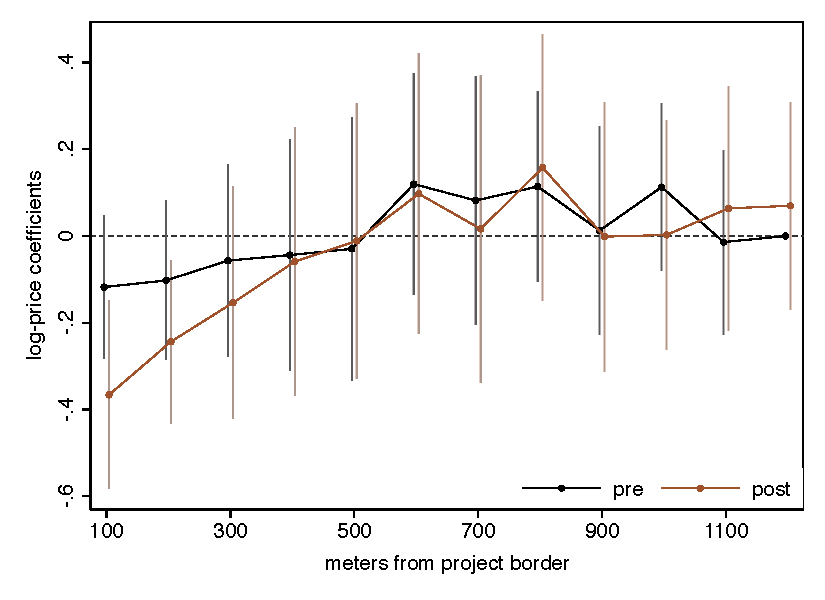
\includegraphics[scale=0.72]{distplot.pdf}
\vspace{-3mm}
\end{figure}
\end{center}
\end{frame}


%------------------------------------------------

\begin{frame}
\frametitle{Placebo Distance Plot}
\begin{center}
\begin{figure}


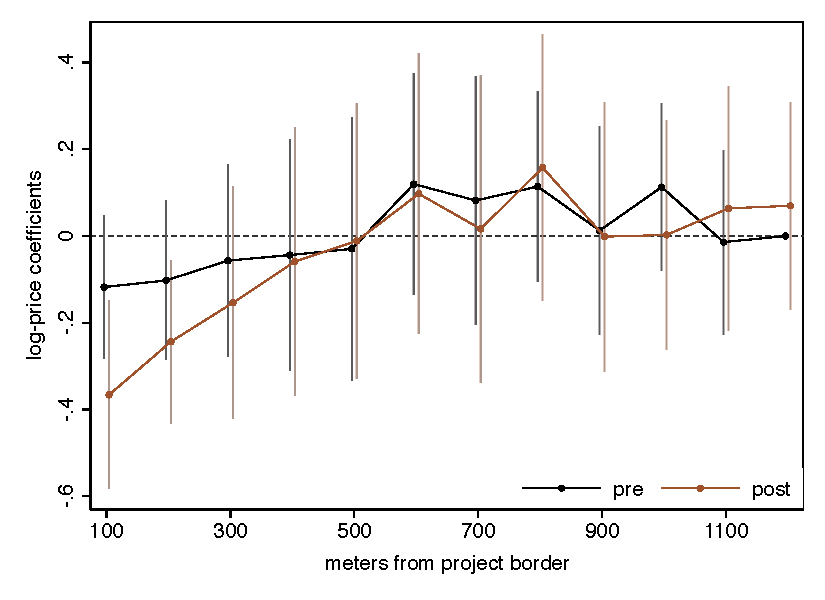
\includegraphics[width=0.5\textwidth,trim={.77cm 0cm .21cm 0cm}]{distplot.pdf}
   \hfill
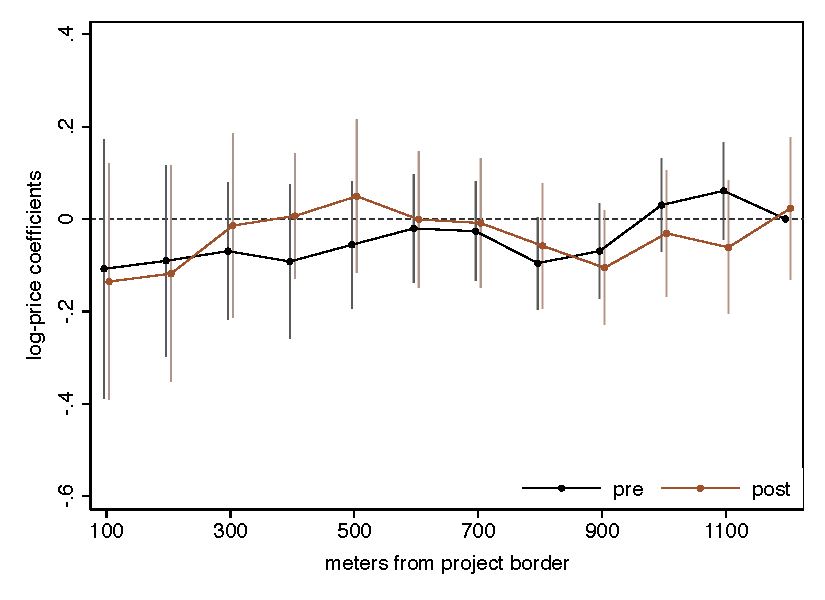
\includegraphics[width=0.5\textwidth,trim={.77cm 0cm .21cm 0cm},clip]{distplot_placebo.pdf}

\end{figure}
\end{center}
\end{frame}

%------------------------------------------------

\begin{frame}
\frametitle{Time Plot}
\begin{center}
\begin{figure}

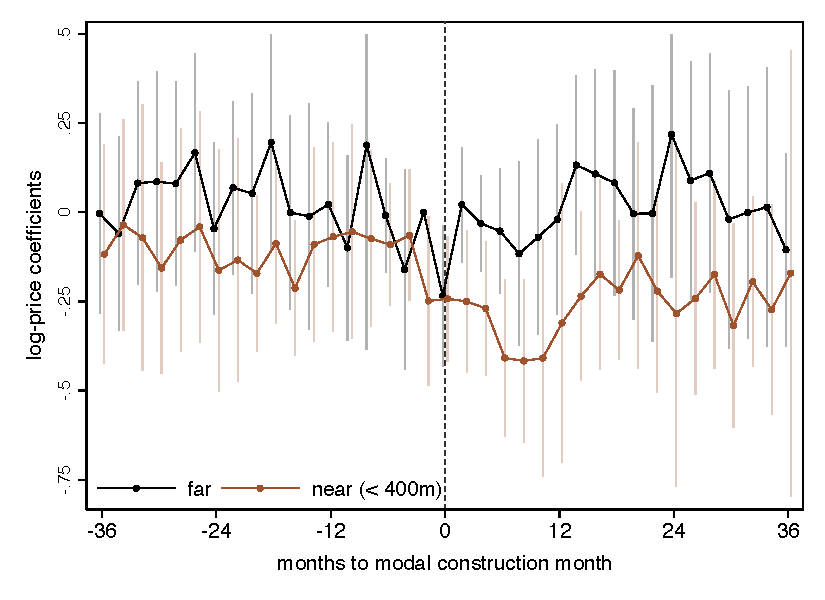
\includegraphics[scale=0.72]{timeplot.pdf}

\end{figure}
\end{center}
\end{frame}

%------------------------------------------------

\begin{frame}
\frametitle{Placlebo Time Plot}
\begin{center}
\begin{figure}

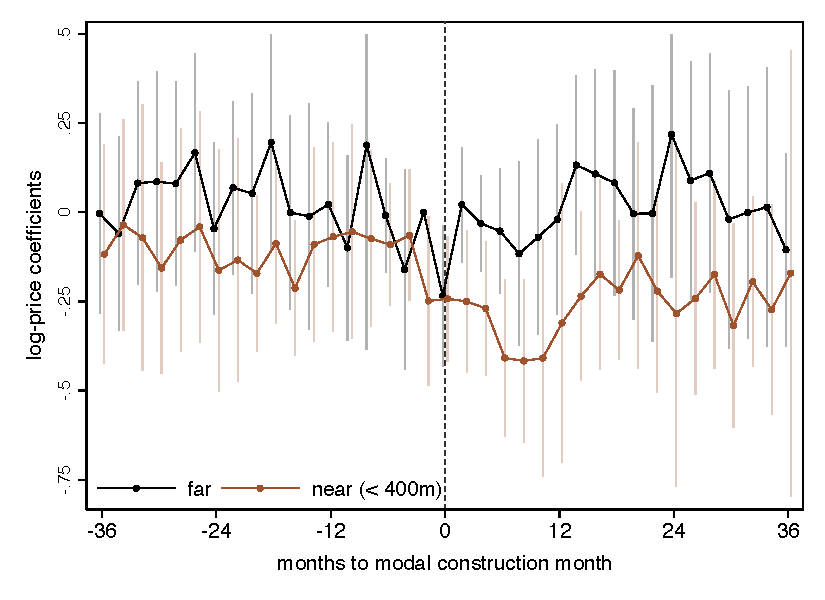
\includegraphics[width=0.5\textwidth,trim={.77cm 0cm .21cm 0cm}]{timeplot.pdf}
   \hfill
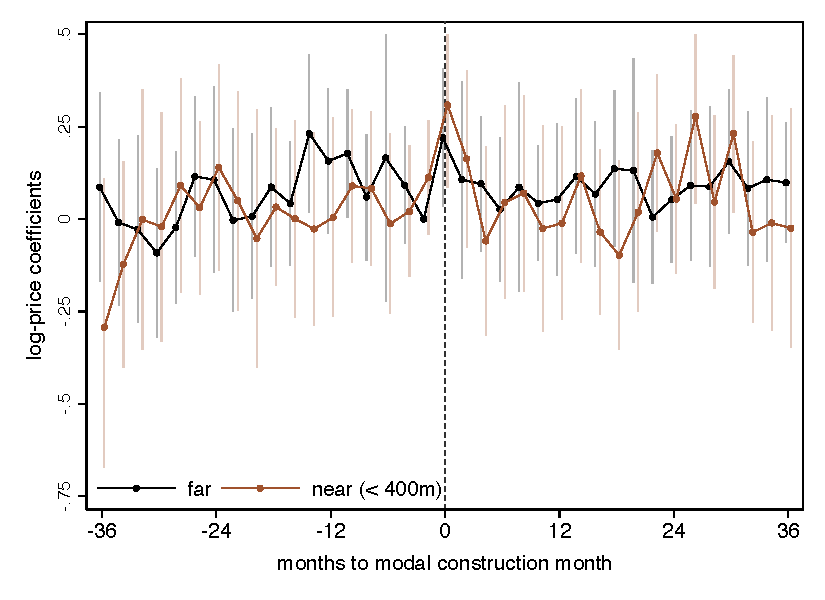
\includegraphics[width=0.5\textwidth,trim={.77cm 0cm .21cm 0cm},clip]{timeplot_placebo.pdf}

\vspace{-3mm}
\end{figure}
\end{center}
\end{frame}

%------------------------------------------------

\begin{frame}
\frametitle{Transaction Densities}
\begin{center}
\begin{figure}
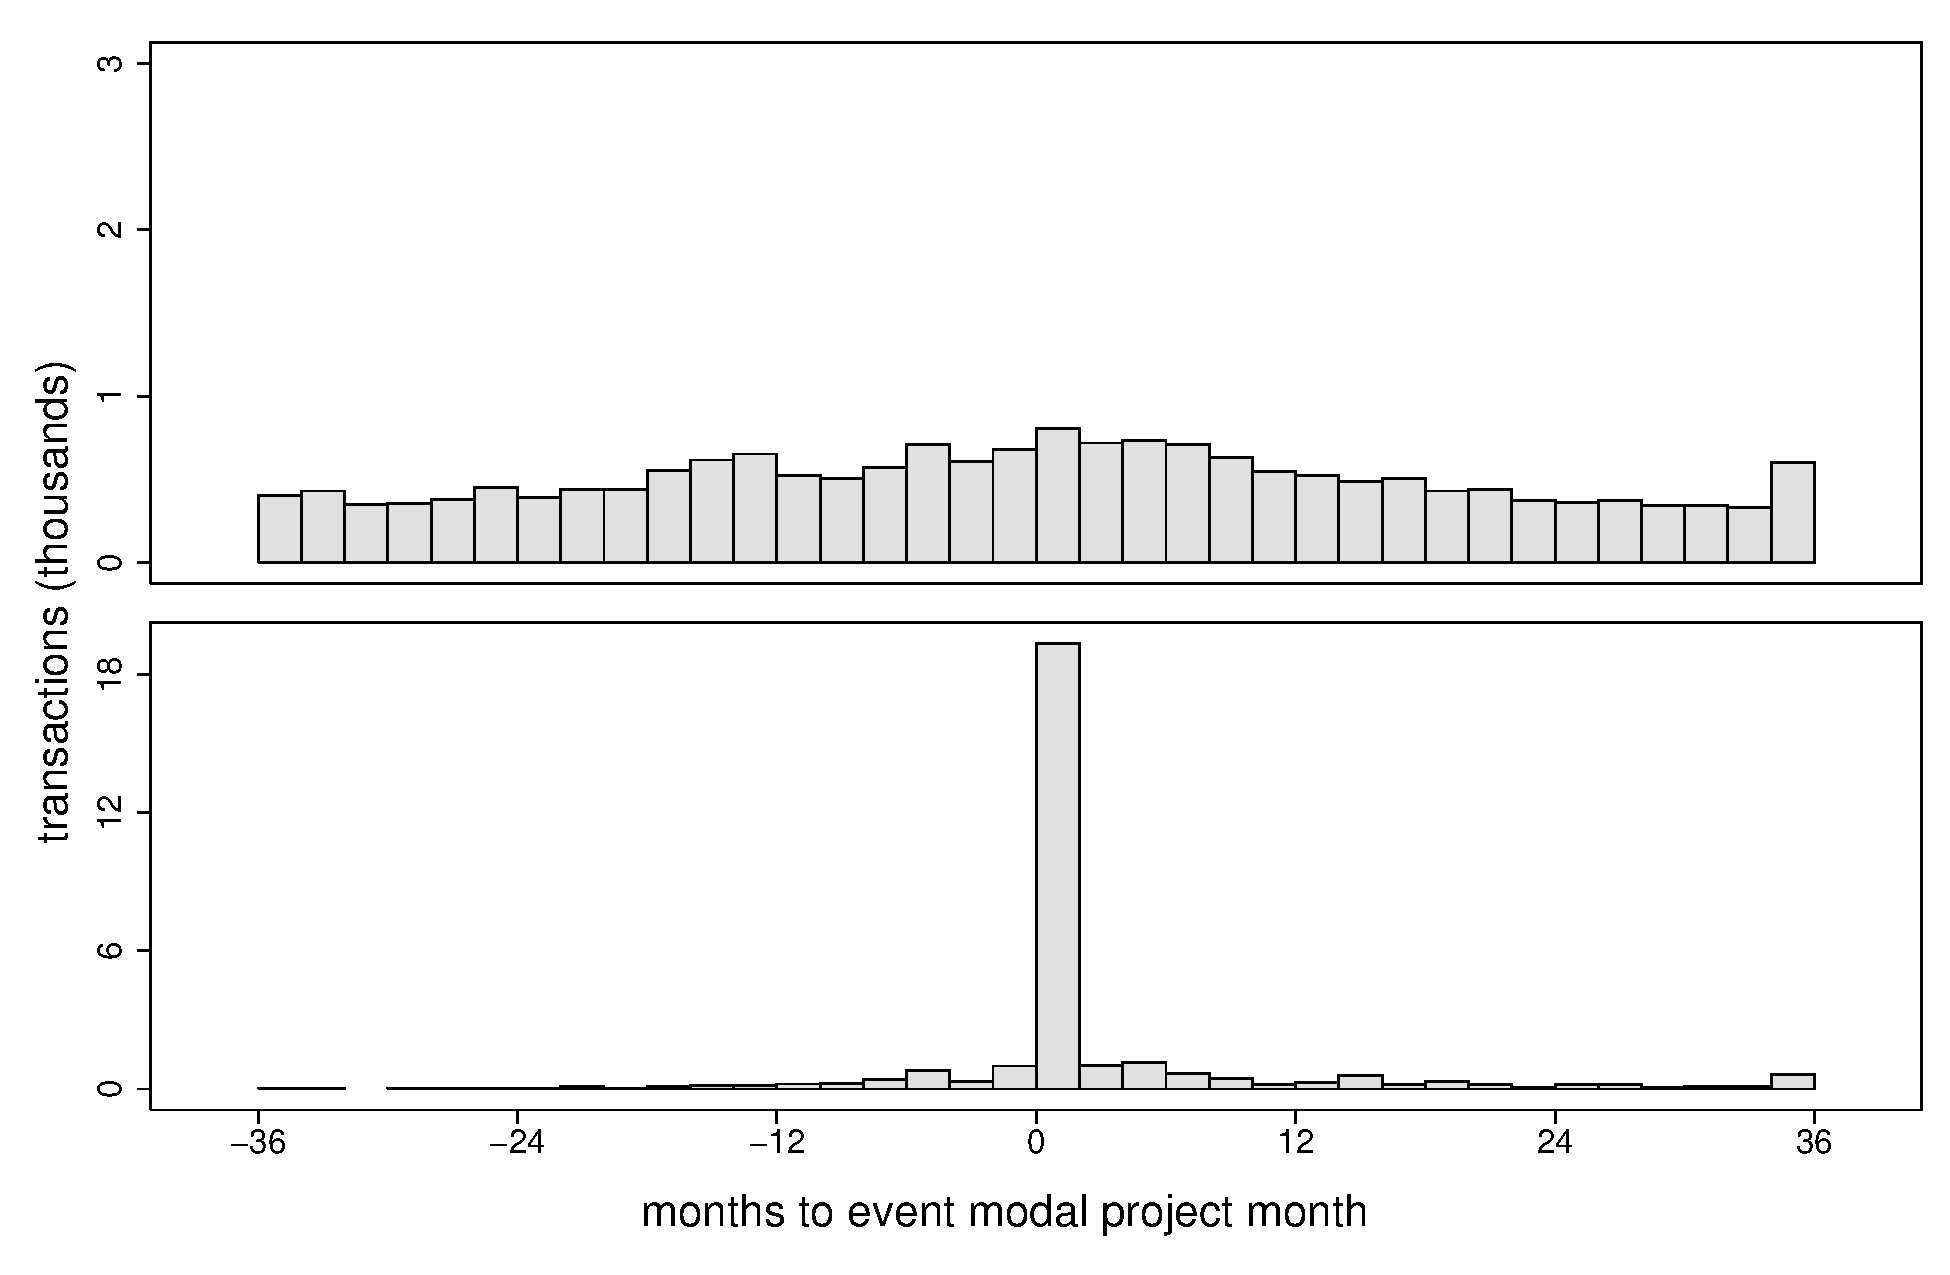
\includegraphics[scale=0.32]{summary_densitytime.pdf}
\vspace{-3mm}
\end{figure}
\end{center}
\end{frame}

%------------------------------------------------

\begin{frame}
\frametitle{Transaction Densities}
\begin{center}
\begin{figure}
\includegraphics[scale=0.72]{rdpvsnonrdp.pdf}
\vspace{-3mm}
\end{figure}
\end{center}
\end{frame}


%------------------------------------------------

\begin{frame}
\frametitle{Housing Projects}
\vspace{-1.5mm}
\begin{table}
{\footnotesize
\begin{tabular}{lcccc} \hline
 & (1) & (2) & (3) & (4) \\
VARIABLES & Log Price & Log Price & Log Price & Log Price \\ \hline
 &  &  &  &  \\
3 yrs 0-400m & -0.238** & -0.166* &  &  \\
 & (0.106) & (0.0835) &  &  \\
1st yr 0-400m &  &  & -0.147* &  \\
 &  &  & (0.0754) &  \\
2nd yr 0-400m &  &  & -0.180 &  \\
 &  &  & (0.115) &  \\
3rd yr 0-400m &  &  & -0.118 &  \\
 &  &  & (0.0971) &  \\
3 yrs 0-200m &  &  &  & -0.224** \\
 &  &  &  & (0.0961) \\
3 yrs 200-400m &  &  &  & -0.0701 \\
 &  &  &  & (0.0664) \\
 &  &  &  &  \\
Observations & 28,701 & 28,701 & 28,701 & 28,701 \\
R-squared & 0.229 & 0.488 & 0.489 & 0.489 \\
Project FE & NO & YES & YES & YES \\
 Year-Month FE & YES & YES & YES & YES \\ \hline
\multicolumn{5}{c}{ Robust standard errors in parentheses} \\
\multicolumn{5}{c}{ *** p$<$0.01, ** p$<$0.05, * p$<$0.1} \\
\multicolumn{5}{c}{ All control for cubic in plot size. Standard errors are clustered at the project level.} \\
\end{tabular}

}
\end{table}
\end{frame}

%------------------------------------------------

\begin{frame}
\frametitle{Housing Projects}
\vspace{-1.5mm}
\begin{table}
{\footnotesize
\begin{tabular}{lcccc} \hline
 & (1) & (2) & (3) & (4) \\
VARIABLES & Log Price & Log Price & Log Price & Log Price \\ \hline
 &  &  &  &  \\
3 yrs 0-400m & -0.0435 & -0.0664 &  &  \\
 & (0.0784) & (0.0597) &  &  \\
1st yr 0-400m &  &  & -0.0687 &  \\
 &  &  & (0.0662) &  \\
2nd yr 0-400m &  &  & 0.00256 &  \\
 &  &  & (0.0729) &  \\
3rd yr 0-400m &  &  & -0.159* &  \\
 &  &  & (0.0841) &  \\
3 yrs 0-200m &  &  &  & -0.0365 \\
 &  &  &  & (0.0739) \\
3 yrs 200-400m &  &  &  & -0.0896 \\
 &  &  &  & (0.0624) \\
 &  &  &  &  \\
Observations & 24,562 & 24,562 & 24,562 & 24,562 \\
R-squared & 0.307 & 0.502 & 0.502 & 0.502 \\
Project FE & NO & YES & YES & YES \\
 Year-Month FE & YES & YES & YES & YES \\ \hline
\multicolumn{5}{c}{ Robust standard errors in parentheses} \\
\multicolumn{5}{c}{ *** p$<$0.01, ** p$<$0.05, * p$<$0.1} \\
\multicolumn{5}{c}{ All control for cubic in plot size. Standard errors are clustered at the project level.} \\
\end{tabular}

}
\end{table}
\end{frame}

%------------------------------------------------

\begin{frame}
\frametitle{Housing Projects}
\vspace{-1.5mm}
\begin{table}
{\footnotesize
{
\def\sym#1{\ifmmode^{#1}\else\(^{#1}\)\fi}
\begin{tabular}{l*{5}{c}}
 & (1) & (2) & (3) & (4) & (5)  \\[0.2em]
\hline\\[-0.9em]

                           &   flush toilet   &   water tap     &   elec. cooking  &   elec. light &  house\\
[0.2em]\hline \\[-0.9em]

DD $>$30\% overlap         &    0.265\sym{**} &  0.241\sym{***} &    0.034         &   -0.029      &    0.207\sym{***}\\
                           &  (0.101)         &  (0.060)        &  (0.107)         &  (0.134)      &  (0.051)         \\
[0.5em]
DD $\leq$30\% overlap      &   -0.027         & -0.070\sym{**}  &   -0.106\sym{**} &   -0.016      &   -0.069\sym{**} \\
                           &  (0.037)         &  (0.033)        &  (0.042)         &  (0.033)      &  (0.032)         \\
\hline \\[-0.9em]    
\(N\)                      &  1,382,550       &  1,382,550      &  1,382,550       &  1,382,550    &  1,329,296         \\
\(R^{2}\)                  &    0.352         &    0.212        &    0.249         &    0.244      &    0.157         \\\hline
\multicolumn{6}{l}{\tiny Standard errors clusterred at the project level. All specifications control for project FE}
\end{tabular}
}

}
\end{table}
\end{frame}

%------------------------------------------------

\begin{frame}
\frametitle{Housing Projects}
\vspace{-1.5mm}
\begin{table}
{\footnotesize
{
\def\sym#1{\ifmmode^{#1}\else\(^{#1}\)\fi}
\begin{tabular}{l*{5}{c}}
 & (1) & (2) & (3) & (4) & (5)  \\[0.2em]
\hline\\[-0.9em]

                           &   flush toilet   &   water tap     &   elec. cooking  &   elec. light &  house\\
[0.2em]\hline \\[-0.9em]

DD $>$30\% overlap         &    0.193\sym{***}&   0.201\sym{***}&    0.156\sym{*}  &    0.060      &    0.235\sym{***}\\
                           &  (0.062)         &  (0.041)        &  (0.086)         &  (0.088)      &  (0.039)         \\
[0.5em]
DD $\leq$30\% overlap      &   -0.027         & -0.070\sym{**}  &   -0.106\sym{**} &   -0.016      &   -0.069\sym{**} \\
                           &  (0.037)         &  (0.033)        &  (0.042)         &  (0.033)      &  (0.032)         \\
\hline \\[-0.9em]    
\(N\)                      &  3,488,910       &  3,488,910      &  3,488,910       &  3,488,910    &  3,322,977         \\
\(R^{2}\)                  &    0.335         &    0.213        &    0.257        &    0.252       &    0.175         \\
\hline
\multicolumn{6}{l}{\tiny Standard errors clusterred at the project level. All specifications control for project FE}
\end{tabular}
}

}
\end{table}
\end{frame}

%------------------------------------------------

\begin{frame}
\frametitle{Housing Projects}
\vspace{-1.5mm}
\begin{table}
{\footnotesize
{
\def\sym#1{\ifmmode^{#1}\else\(^{#1}\)\fi}
\begin{tabular}{l*{3}{c}}
 & (1) & (2) & (3)  \\[0.2em]
\hline\\[-0.9em]

                           &   high-school    &   monthly income     &   unemployed  \\
[0.2em]\hline \\[-0.9em]

DD $>$30\% overlap         &  -0.053\sym{***}  &  226.330         &   -0.008         \\
                           &  (0.013)          &(372.469)         &  (0.023)         \\
[0.5em]
DD $\leq$30\% overlap      &   -0.008         &   77.967         &    0.024         \\
                           &  (0.012)         &(428.078)         &  (0.016)         \\
\hline \\[-0.9em]    
\(N\)                      &  2,055,289         &   909,466         &  1,069,857    \\
\(R^{2}\)                  &    0.024         &    0.050         &    0.049         \\
\hline
\multicolumn{4}{l}{\tiny Standard errors clusterred at the project level. All specifications control for project FE}
\end{tabular}
}

}
\end{table}
\end{frame}

%------------------------------------------------

\begin{frame}
\frametitle{Housing Projects}
\vspace{-1.5mm}
\begin{table}
{\footnotesize
{
\def\sym#1{\ifmmode^{#1}\else\(^{#1}\)\fi}
\begin{tabular}{l*{3}{c}}
 & (1) & (2) & (3)  \\[0.2em]
\hline\\[-0.9em]

                           &   high-school    &   monthly income     &   unemployed  \\
[0.2em]\hline \\[-0.9em]

DD $>$30\% overlap         &  -0.030\sym{***} &  341.461         &   -0.011         \\
                           &  (0.011)         &  (308.922)       &  (0.012)         \\
[0.5em]
DD $\leq$30\% overlap      &    -0.006        &  273.137         &    0.009         \\
                           &  (0.007)         & (296.929)        &  (0.009)         \\
\hline \\[-0.9em]    
\(N\)                      &  5,103,934       &  2,279,500       &  2,734,902       \\
\(R^{2}\)                  &    0.022         &    0.058         &    0.056         \\
\hline
\multicolumn{4}{l}{\tiny Standard errors clusterred at the project level. All specifications control for project FE}
\end{tabular}
}

}
\end{table}
\end{frame}

%------------------------------------------------

\begin{frame}
\frametitle{BBLU plot}
\begin{center}
\begin{figure}
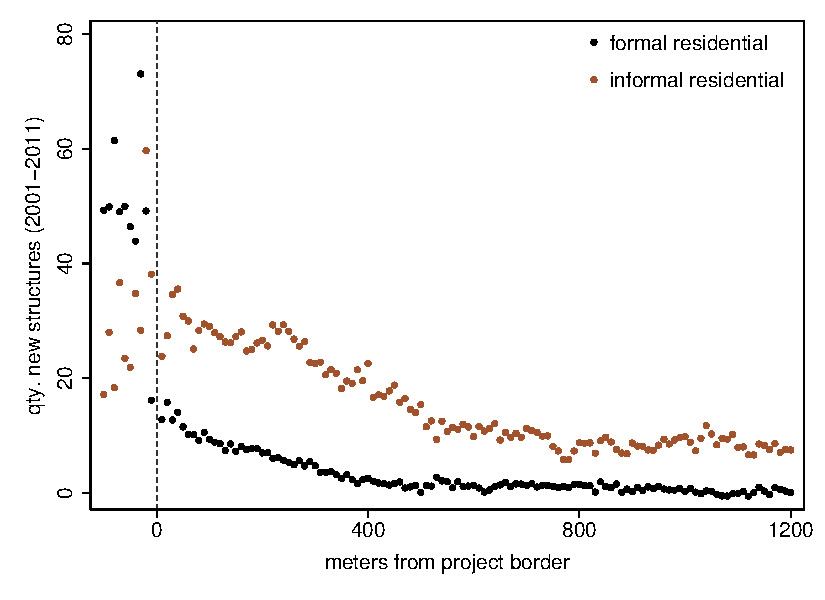
\includegraphics[scale=0.72]{bbluplot.pdf}
\vspace{-3mm}
\end{figure}
\end{center}
\end{frame}


%------------------------------------------------

\begin{frame}
\frametitle{BBLU plot placebo}
\begin{center}
\begin{figure}

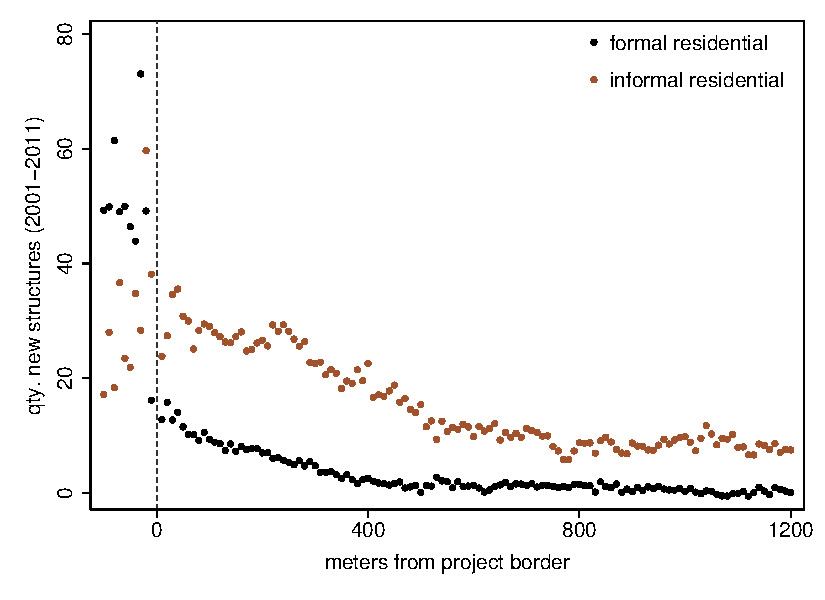
\includegraphics[width=0.5\textwidth,trim={.75cm 0cm .21cm 0cm}]{bbluplot.pdf}
   \hfill
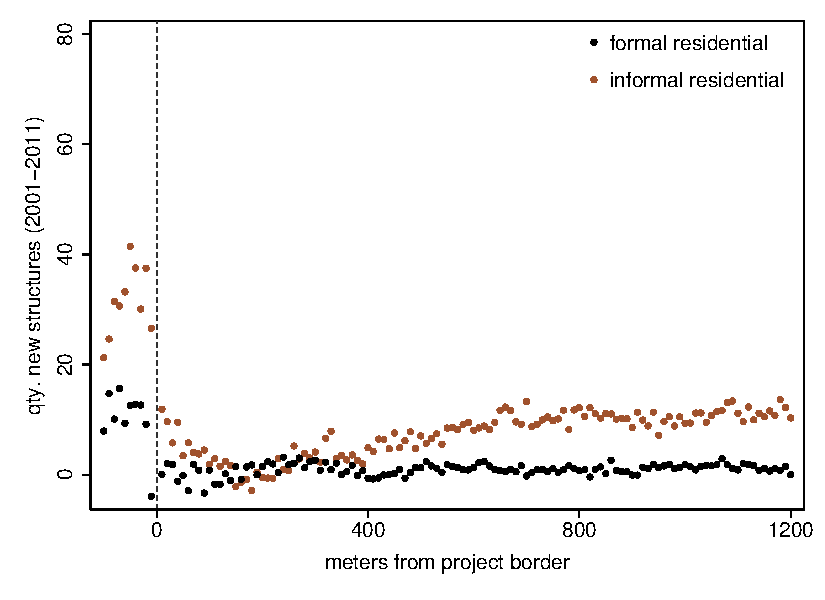
\includegraphics[width=0.5\textwidth,trim={.75cm 0cm .21cm 0cm},clip]{bbluplot_placebo.pdf}

\end{figure}
\end{center}
\end{frame}


%------------------------------------------------






\end{document} 
